% Created 2024-05-21 Tue 09:26
% Intended LaTeX compiler: pdflatex
\documentclass[presentation]{beamer}
\usepackage{luatexja}

                 \usepackage{luatexja}
                 \usepackage{luatexja-preset}
\usetheme{Madrid}
\usecolortheme{beetle}
\author{Atsushi Odagiri}
\date{2024-04-25}
\title{パッケージを配ろう}
\hypersetup{
 pdfauthor={Atsushi Odagiri},
 pdftitle={パッケージを配ろう},
 pdfkeywords={},
 pdfsubject={},
 pdfcreator={Emacs 29.3 (Org mode 9.6.15)}, 
 pdflang={English}}
\begin{document}

\maketitle
\begin{frame}{Outline}
\tableofcontents
\end{frame}

\section{パッケージを配ろう}
\label{sec:org31595d1}
\begin{frame}[label={sec:org90ce0fb}]{お前誰よ}
\begin{block}{}
\begin{itemize}
\item Atsushi Odagiri
\item Open Collector
\item Pythonは1.5くらいのころから
\end{itemize}
\end{block}

\begin{block}{}
\begin{center}
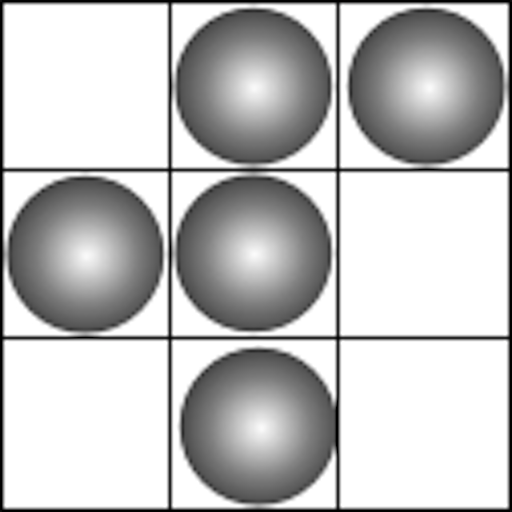
\includegraphics[width=2cm]{./r-penta512.png}
\end{center}

\begin{center}

\includegraphics[width=2cm]{./oc-logo.png}
\end{center}
\begin{center}

\includegraphics[width=2cm]{./logo-w.png}
\end{center}
\end{block}
\end{frame}
\section{パッケージを配るということ}
\label{sec:org790f4bd}
\begin{frame}[label={sec:org67619a1}]{パッケージエコシステム}
\begin{itemize}
\item 作る
\item 配る
\item 使う
\end{itemize}
\end{frame}

\begin{frame}[label={sec:orgf3f5b2c}]{パッケージを配るということ}
\begin{itemize}
\item 広く一般に向けて配る
\item 狭い範囲で限られた利用のために配る
\end{itemize}
\end{frame}

\begin{frame}[label={sec:orgc3e8cd1},fragile]{広く一般に向けてpypiで配る}
 \begin{itemize}
\item PyPAツールのデフォルト
\item \texttt{tween} でアップロード
\item \texttt{pip} がダウンロードしてインストール
\end{itemize}
\end{frame}

\begin{frame}[label={sec:org3c4ede4}]{狭い範囲で限られた利用のために配る}
\begin{itemize}
\item マイクロサービスのそれぞれて使うようなライブラリ
\item 特殊なパッチをあてたローカルフレーバーライブラリ
\end{itemize}
\end{frame}

\begin{frame}[label={sec:org897a986}]{狭い範囲で配る}
\begin{itemize}
\item 社内ネットワークやVPNの中で
\item k8sやvpcの中で
\item 範囲内のIPアドレスにだけ
\item 認証をつけたい
\end{itemize}
\end{frame}

\section{パッケージを配るためのPEP}
\label{sec:orgfec5d98}
\begin{frame}[label={sec:org9298f5d}]{パッケージを配るためのPEP}
\begin{itemize}
\item \href{https://peps.python.org/pep-0458}{PEP 458 – Secure PyPI downloads with signed repository metadata}
\item \href{https://peps.python.org/pep-0480}{PEP 480 – Surviving a Compromise of PyPI: End-to-end signing of packages}
\item \href{https://peps.python.org/pep-0503/}{PEP 503 – Simple Repository API}
\item \href{https://peps.python.org/pep-0592}{PEP 592 – Adding “Yank” Support to the Simple API}
\item \href{https://peps.python.org/pep-0629}{PEP 629 – Versioning PyPI’s Simple API}
\item \href{https://peps.python.org/pep-0658}{PEP 658 – Serve Distribution Metadata in the Simple Repository API}
\item \href{https://peps.python.org/pep-0691}{PEP 691 – JSON-based Simple API for Python Package Indexes}
\item \href{https://peps.python.org/pep-0700}{PEP 700 – Additional Fields for the Simple API for Package Indexes}
\item \href{https://peps.python.org/pep-0714}{PEP 714 – Rename dist-info-metadata in the Simple API}
\end{itemize}
\end{frame}
\begin{frame}[label={sec:org78be1f3}]{Simple Repository}
\end{frame}
\begin{frame}[label={sec:org0c5fd5e},fragile]{Metadata}
 \begin{itemize}
\item wheelの中にある \texttt{Metadata}
\end{itemize}
\end{frame}
\begin{frame}[label={sec:org92c539f}]{JSON}
\begin{itemize}
\item やることが多い!
\end{itemize}
\end{frame}
\begin{frame}[label={sec:org02ee95c}]{PyPIのSimple Repository}
\begin{itemize}
\item \url{https://pypi.org/simple/} とても大きいのでアクセス注意!
\end{itemize}
\end{frame}
\begin{frame}[label={sec:org7625a11}]{pipでsimple repositoryを使う}
\end{frame}

\section{実践package repository}
\label{sec:org4665011}
\begin{frame}[label={sec:orga2b5165},fragile]{httplib.server でのお手軽repository}
 \begin{itemize}
\item ダウンロードできるリンクがあればいいので \texttt{http} モジュールでサーバーを起動するだけ
\item wheelファイルのあるディレクトリで実行
\end{itemize}

\begin{verbatim}
python3 -m pip download pyramid
python3 -m http.server
pip install pyramid -f http://localhost:8000/ --no-index
\end{verbatim}

\begin{center}
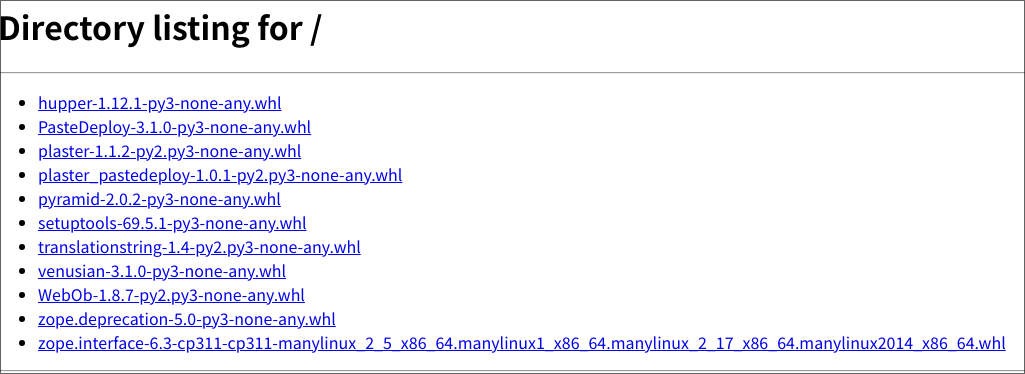
\includegraphics[width=.9\linewidth]{./http-server-simple-repository.png}
\end{center}
\end{frame}

\begin{frame}[label={sec:org023993d}]{wsgi app}
\begin{itemize}
\item webアプリケーションにする
\item DBなどを使わず起動するだけで使える
\end{itemize}
\end{frame}

\begin{frame}[label={sec:org673c19d},fragile]{wheelファイルを探しだす}
 \begin{itemize}
\item wheelファイルのファイル名は形式が決まっている
\texttt{\{distribution\}-\{version\}(-\{build tag\})?-\{python tag\}-\{abi tag\}-\{platform tag\}.whl.}
\end{itemize}
\end{frame}

\begin{frame}[label={sec:org39861ad}]{pypi version}
\begin{itemize}
\item 今回はv1.0の範囲でやってみます

\begin{itemize}
\item PEP691 v1.0
\item PEP714 v1.1
\end{itemize}
\end{itemize}
\end{frame}

\begin{frame}[label={sec:org47a7336},fragile]{metadata}
 \begin{itemize}
\item METADATAをwheelから取り出す
\end{itemize}
\begin{verbatim}
def get_metadata(whl: pathlib.Path):
    parts = whl.name.split("-")
    dist_name, version = parts[0], parts[1]
    metadata_path = f"{dist_name}-{version}.dist-info/METADATA"
    with zipfile.ZipFile(whl) as zf:
        with zf.open(metadata_path) as metadata:
            return metadata.read()

\end{verbatim}
\end{frame}
\begin{frame}[label={sec:org8ae0e17}]{jsonに対応}
\begin{itemize}
\item project list
\item project detail
\end{itemize}
\end{frame}

\begin{frame}[label={sec:orge7fc8f8},fragile]{project list}
 \begin{itemize}
\item v1.0は \texttt{name} のみ
\end{itemize}

\begin{verbatim}
Project = TypedDict("Project", {"name": str})
ProjectList = TypedDict(
    "ProjectList",
    {
        "meta": Meta,
        "projects": list[Project],
    },
)

\end{verbatim}
\end{frame}

\begin{frame}[label={sec:org1e8a099},fragile]{project detail}
 \begin{verbatim}
ProjectDetail = TypedDict(
    "ProjectDetail",
    {
        "name": str,
        "files": list[ProjectFile],
        "meta": Meta,
    },
)

\end{verbatim}
\end{frame}

\begin{frame}[label={sec:orge03022b},fragile]{project file}
 \begin{itemize}
\item すごく情報量が増えた
\end{itemize}

\begin{verbatim}
ProjectFile = TypedDict(
    "ProjectFile",
    {
        "filename": str,
        "url": str,
        "hashes": dict[str, str],
        "requires-python": NotRequired[str],
        "dist-info-metadata": NotRequired[str],
        "gpg-sig": NotRequired[bool],
        "yanked": NotRequired[bool],
    },
)

\end{verbatim}
\end{frame}
\begin{frame}[label={sec:orgee3d345}]{pipから使う}
\begin{itemize}
\item project list呼ばれてないかも?
\end{itemize}
\end{frame}

\begin{frame}[label={sec:orgef6b34d},fragile]{find-links vs index-url}
 \begin{verbatim}
$ pip install pyramid --index-url=http://localhost:8000/
\end{verbatim}
\end{frame}

\begin{frame}[label={sec:orgbffd197}]{The Update Framework}
\begin{itemize}
\item TUF
\end{itemize}
\end{frame}

\section{参考文献}
\label{sec:org0e65395}
\begin{frame}[label={sec:org7413a67}]{参考文献}
\begin{itemize}
\item PyPA Simple Repository API, \url{https://packaging.python.org/en/latest/specifications/simple-repository-api/}
\item The Update Framework, \url{https://theupdateframework.io/}
\end{itemize}
\end{frame}
\end{document}
